\section{\MakeUppercase{Literature Reviews}} \label{chap:one}
This chapter presents the evolution of research on \gls{dnn} in acoustics and its application to event detection, environmental monitoring, etc. Section \ref{sec:fe_and_dnn} examines the progression of audio usage in \gls{ai}, focusing on time-frequency feature extraction methods and \gls{dnn} learning models based on \gls{cnn} and attention mechanisms. Section \ref{sec:acc_mon} outlines \dots

\subsection{Audio Feature Extraction and Deep Neural Networks for Acoustic Classification}\label{sec:fe_and_dnn}
\begin{figure}[!ht]
    \centering
    \begin{subfigure}[b]{0.45\textwidth}
	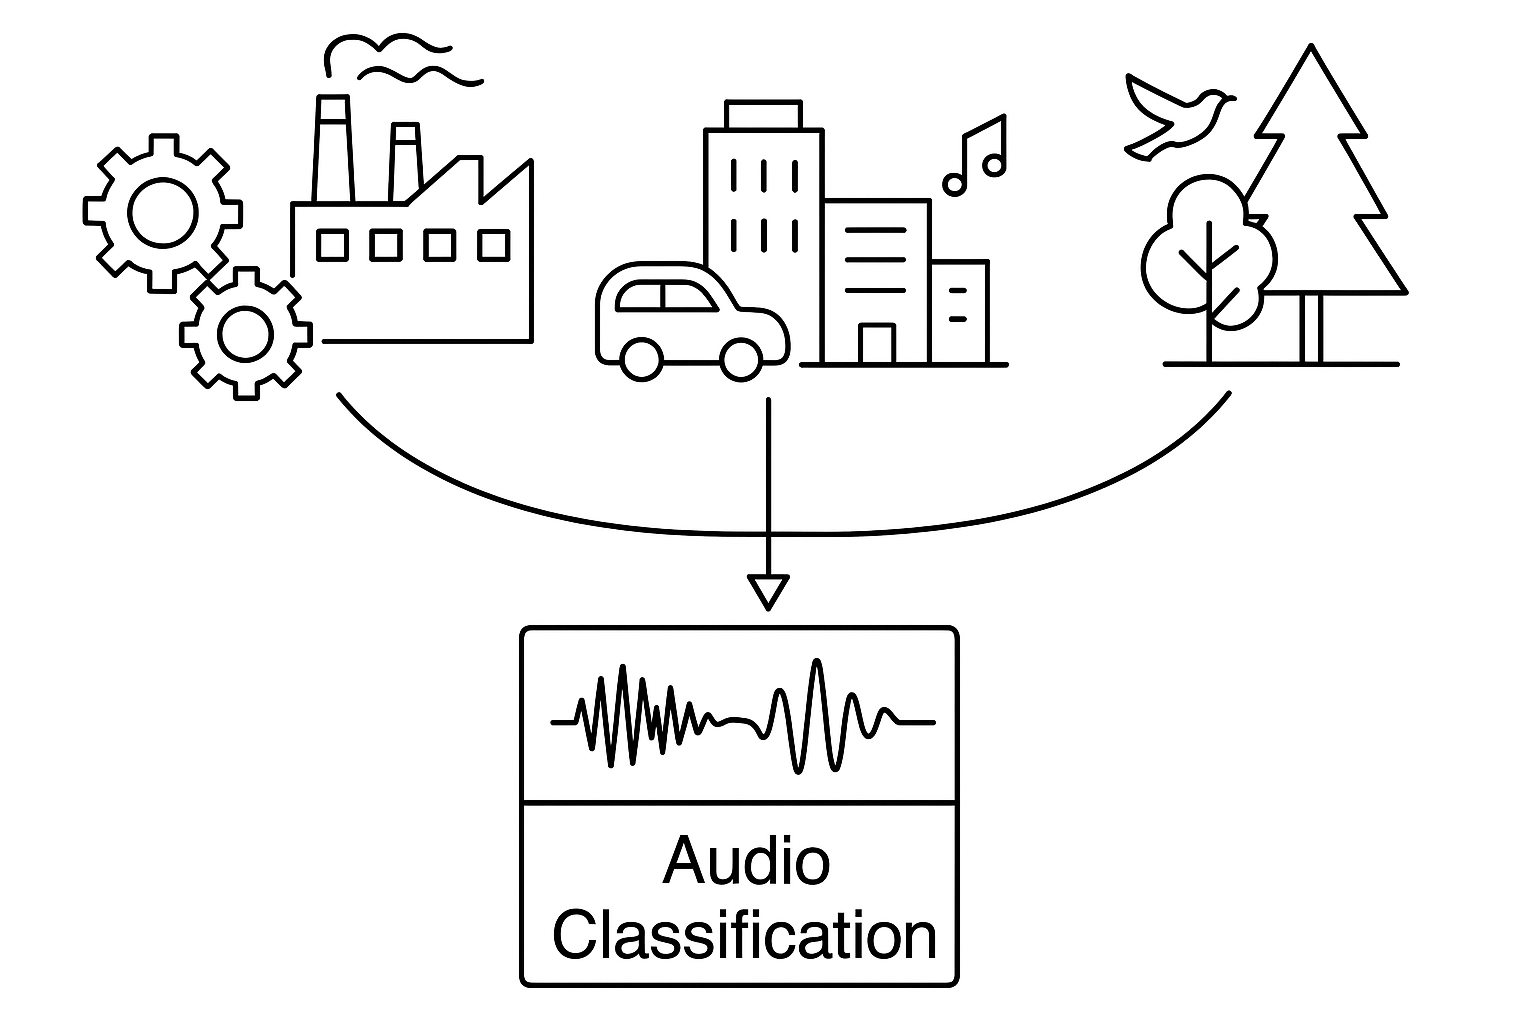
\includegraphics[width=\textwidth]{images/sketch/audioclassification.png}
	\caption{sketch}
	\label{fig:audio-based}
\end{subfigure}
\hfill
\begin{subfigure}[b]{0.45\textwidth}
	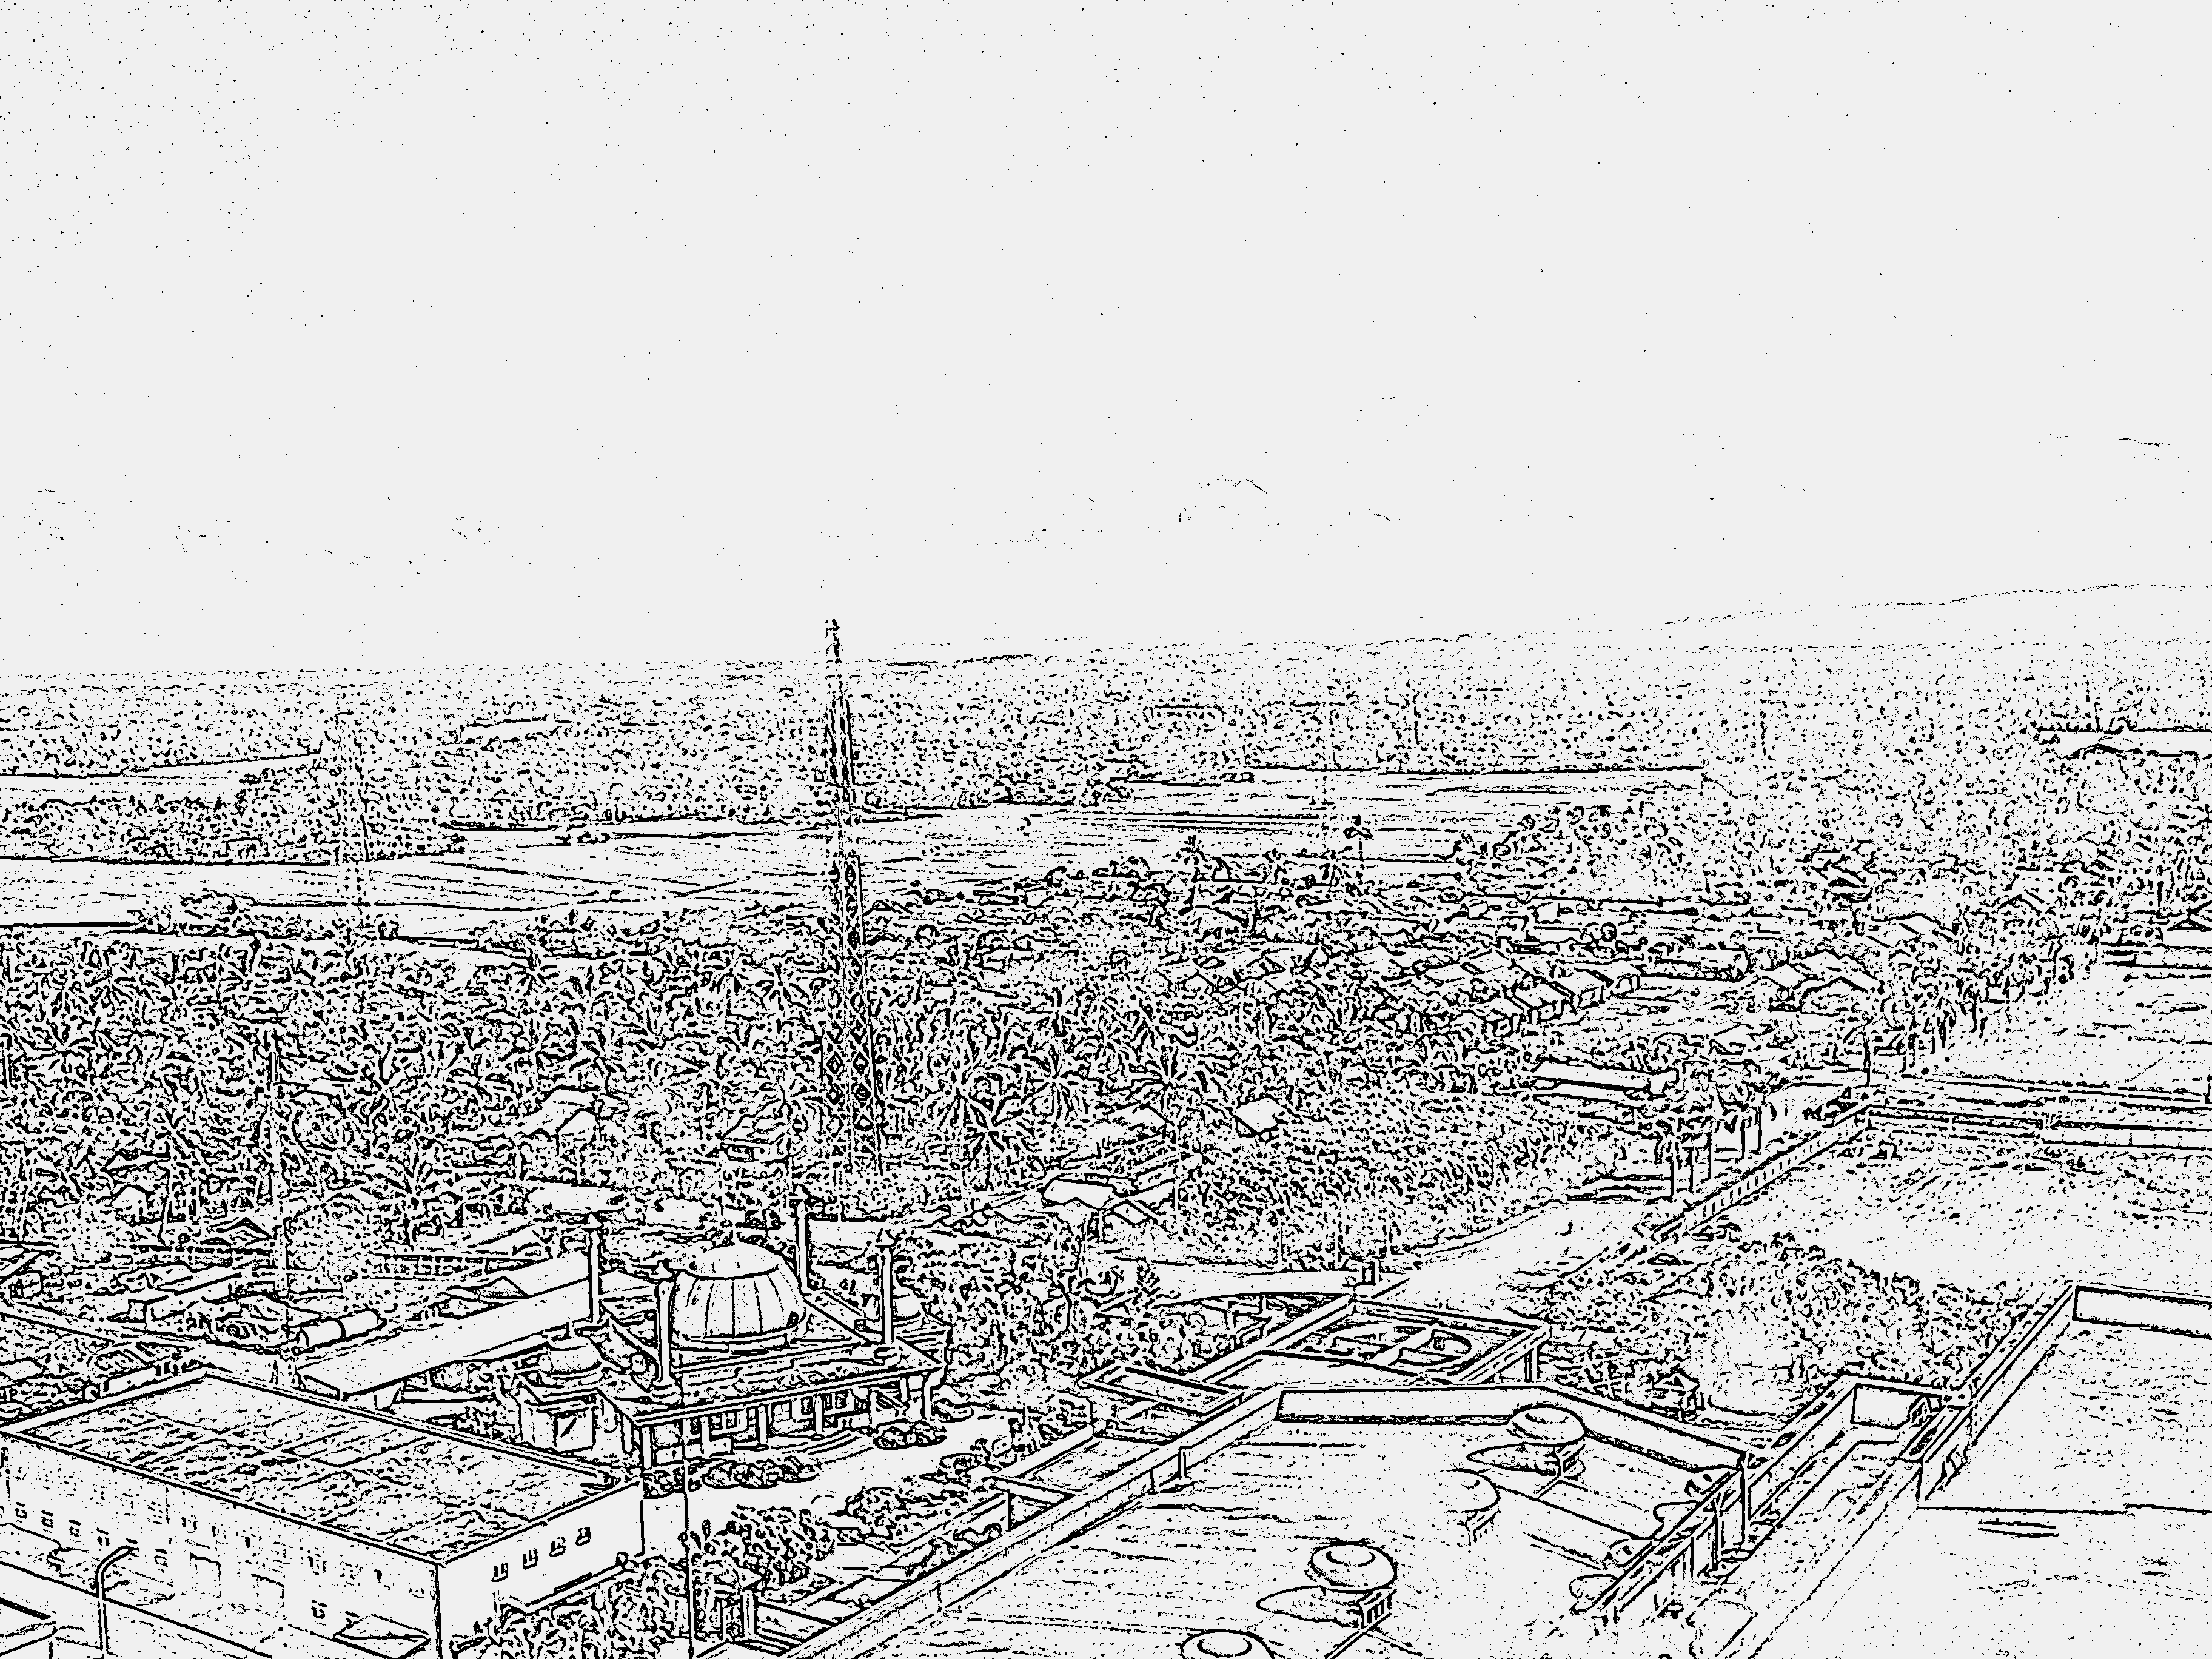
\includegraphics[width=\linewidth]{images/sketch/all_environment_sketch.png}
	\caption{real environment}
	\label{fig:audio_based}
\end{subfigure}
    \caption{Illustration of the implementation of audio-driven classification}
    \label{fig:illustration}
\end{figure}

A combined analysis of advances in \gls{ai} methods and new datasets is essential for \dots

\dots

These developments unlock the potential to broaden the scope of audio classification, enabling both the detection of specific anomalies in varied applications and the identification of unexpected events in real environments. Figure~\ref{fig:illustration} provides \dots


\subsection{Acoustic Monitoring in Noise: Application Areas, Noise Profiles, and Anomaly Definition} \label{sec:acc_mon}
The utilization of acoustic methods in the context of environmental surveillance or the identification of irregularities, as illustrated in Figure~\ref{fig:audio_based}, boasts a substantial historical precedent~\cite{Simonovic2021, Vicuna2017}. In general, abnormal conditions that occur at the measuring device or location can be detected by \dots

\dots

\subsection{Evolution of Acoustic Anomaly Detection Research: A Review Perspective} \label{sec:evo_and}
The merging of acoustic methods with the progress in \gls{ai} has garnered growing attention from researchers, particularly in their use for anomaly detection. The timeline of progress in this interdisciplinary area is detailed through multiple reviews (\gls{tlr}, \gls{slr}, \gls{mlr}, \gls{nlr}, \gls{etc}) that together explain the development, usage, and effectiveness of these techniques in different fields. Table~\ref{tab:recent_literature_reviews} offers a compiled overview of these important reviews.

\glsunset{dtl}
\begin{table}[!ht]
	\centering
	\caption{Recent literature reviews in acoustic-based detections}
	\label{tab:recent_literature_reviews}
    \small
	\begin{tabular}{p{0.3\linewidth}ccp{0.4\linewidth}}
		\toprule
		\multicolumn{1}{c}{Author(s)}&\multicolumn{1}{c}{Method}&Citations&\multicolumn{1}{c}{Focus of study}\\
		\midrule
		Shaikh \gls{etal} (2021)~\cite{Shaikh2021} & \gls{tlr} & 44 & Exploring the potential of acoustic signal analysis in facilitating machine fault diagnosis.\\
		\hline
		Qurthobi \gls{etal} (2022)~\cite{Qurthobi2022}& \gls{slr} & 52 & \Gls{sota} mechanical failure detection using acoustic methods.\\
		\hline
		\dots& \dots & \dots & \dots\\
		\bottomrule
	\end{tabular}
\end{table}
\glsreset{dtl}
\dots
